\section{Results}\label{sec:results}

\subsection{Benchmarks}\label{sec:results:benchmark}
\todo{30 out of 96 benchmarks improve by 5 percent}
\begin{table}
    \centering
    \csvautobooktabular{data/results.csv}
    \caption{Results of 30 improved benchmarks from ISCAS'85, LGSynth'91, and EPFL}\label{tab:results}
\end{table}
\subsection{Marginal Improvement}\label{sec:results:margin}
\todo{graph showing improvement with iter count}
\begin{figure}
    \centering
    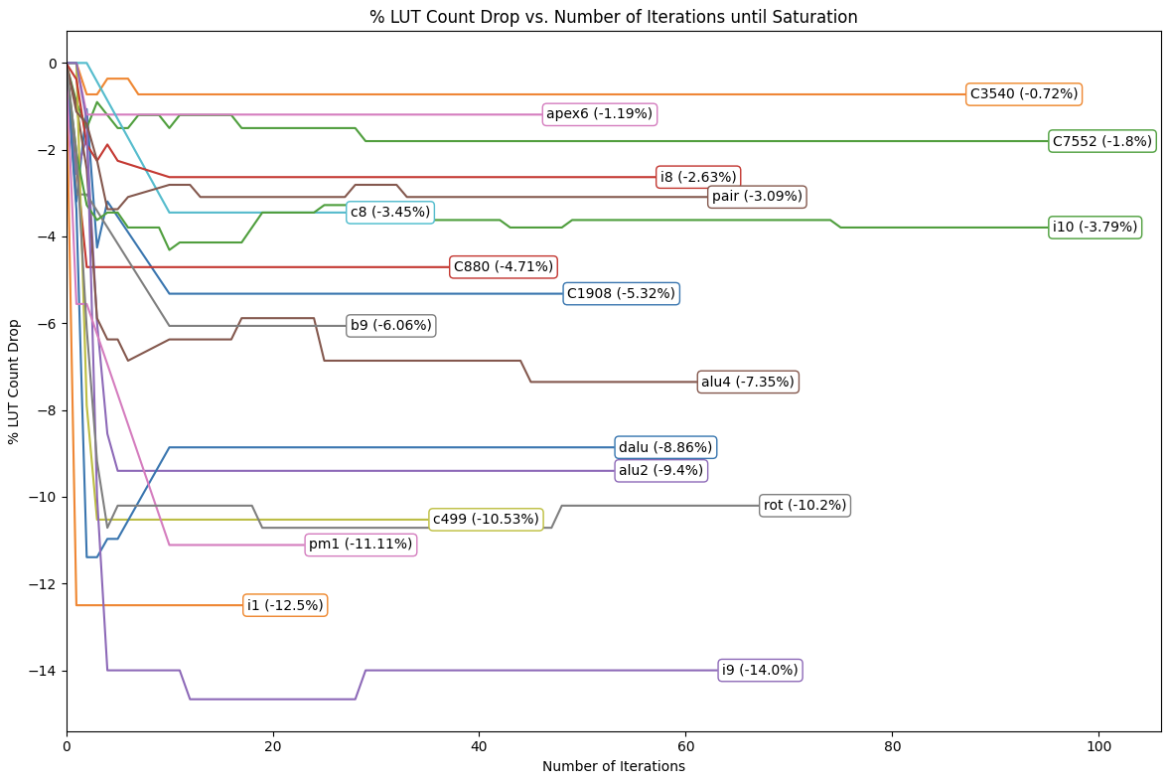
\includegraphics[width=0.47\textwidth]{img/improvement.png}
    \caption{Marginal improvement versus iteration count.}\label{fig:improvement}
    \Description[]{}
\end{figure}

\subsection{Pipelined Designs}\label{sec:results:retiming}
\todo{pipelined mult design}

\subsection{Bit-Parallel Designs}\label{sec:results:scalability}
\todo{increasing ALU bit parallelism}

\subsection{Runtime Complexity}\label{sec:results:complexity}
\todo{graph showing marginal runtime cost of each iteration}
\begin{figure}
    \centering
    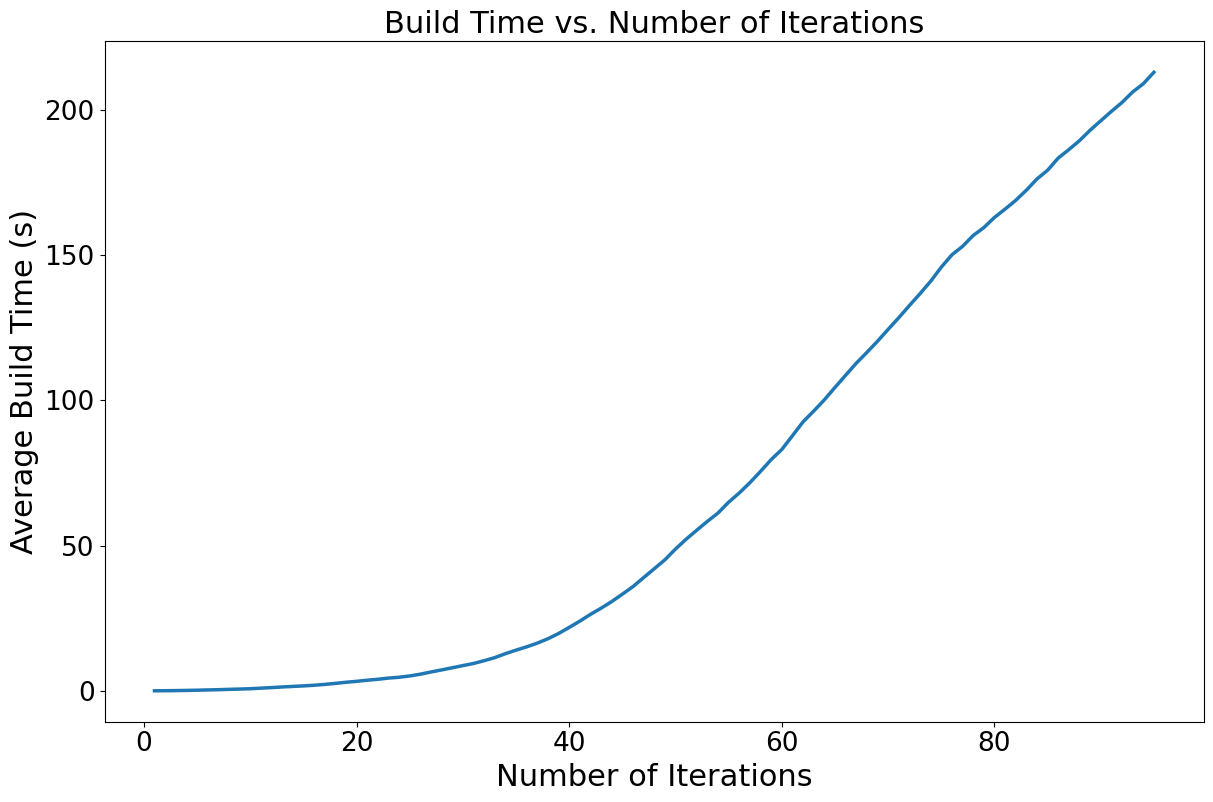
\includegraphics[width=0.47\textwidth]{img/runtime.png}
    \caption{Marginal increase in runtime versus iteration count.}\label{fig:runtime}
    \Description[]{}
\end{figure}